\section{2Nx Interleaved Boost Converter}\label{ch:2Nx}

\todo[color=c04y,inline]{testing the colors}

The final topology presented is the 2Nx Interleaved Boost Converter, which can be achieved by adding a Non-inverting Nx Multilevel BC with a negative Inverting Nx Multilevel BC as presented on Figure~\ref{fig:MBC_2NxDiagram}

\begin{figure}[H]
   \centering
   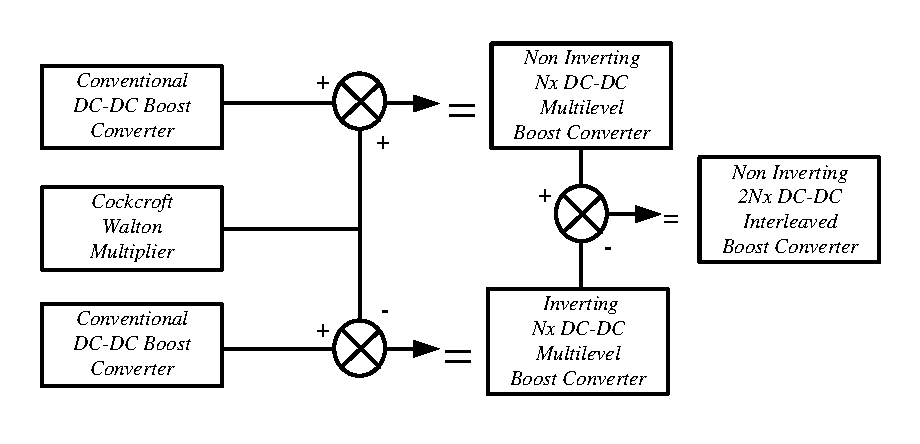
\includegraphics[width=\textwidth]{figures/yMultilevel/2Nx_Diagram.pdf}
    \caption{2Nx Interleaved Boost Converter Diagram}
	\label{fig:MBC_2NxDiagram}
\end{figure}

\subsubsection{Principle of operation}

The 2Nx Interleaved Boost Converter works in a similar way as the Non-inverting Nx and Inverting Nx Multilevel Boost Converters presented in Sections~\ref{ch:MBC} and~\ref{ch:IMBC} respectively. As the two topologies are combined, the voltage gain is increased two times.

The corresponding schematic of the Non-inverting 2Nx Interleaved Boost Converter can be observed on Figure~\ref{fig:MBC_2NxSchematic}. This topology requires 4N - 1 capacitors, 4N - 1 diodes, 2 inductors and 2 switches. Higher number of levels can be achieved by adding additional capacitors and diodes as presented on the schematic in order to increase the voltage gain.

\begin{figure}[H]
   \centering
   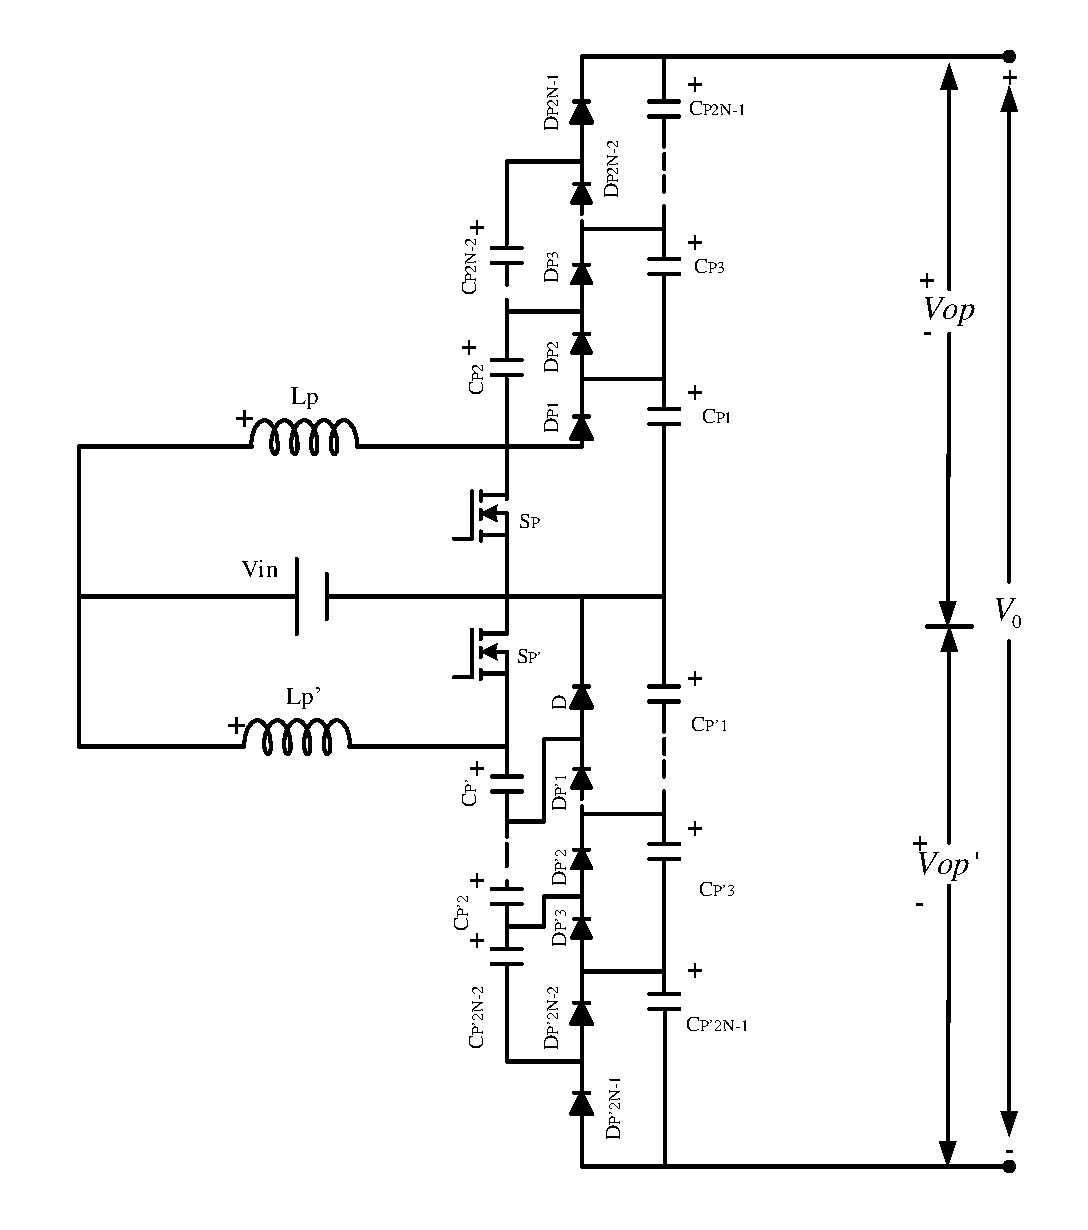
\includegraphics[width=\textwidth]{figures/yMultilevel/2Nx_full.pdf}
    \caption{2Nx Interleaved Boost Converter Schematic}
	\label{fig:MBC_2NxSchematic}
\end{figure}

\subsubsection{Conversion ratio}

As the 2Nx Interleaved Boost Converter is a combination of Non-inverting and Inverting Multilevel Boost Converters, we have $\frac{N}{1-D}$ for the top part and $\frac{N}{1-D}$ for the bottom part of the schematic, which means that the total output-input voltage ratio is:

\begin{equation}
	\frac{V_o}{V_{in}} = \frac{2N}{(1-D)}
	\label{eq:MBC_2NxCR}
\end{equation}

\subsubsection{Simulation}

In order to verify that the conversion ratio is correct,
the topology was built on Simulink. 
Again, the same parameters for the components were used as the other topologies as observed on Table~\ref{tab:MBC_2Nx}.

\begin{table}[H]
\begin{center}
\caption {Simulation parameters for MBC} \label{tab:MBC_2Nx} 
\begin{tabular}{|l|l|}
\cline{1-2}
\textbf{Parameter} & \textbf{Value}  \\ \cline{1-2}
Input Voltage $V_{in}$          &      10V   \\ \cline{1-2}
Load(R)   & 225$\Omega$           \\ \cline{1-2}
Capacitance(C)          &       220$\mu$F     \\ \cline{1-2}
Inductance(L)          &      150$\mu$F      \\ \cline{1-2}
Duty cycle(D)          &     0.6       \\ \cline{1-2}
Switching Frequency($F_S$)          &      50kHz      \\ \cline{1-2}
\end{tabular}
\end{center}
\end{table}

For a 6 level Boost Converter with a duty cycle of 0.6, the expected voltage output gain is

\begin{equation}
	\frac{2\cdot N}{1-D} = \frac{6}{1-D}  = 15
\end{equation}

We can see that the simulation result verifies the calculated conversion ratio on Figure~\ref{fig:MBC_2NxSimResult}. 

\begin{figure}[H]
   \centering
   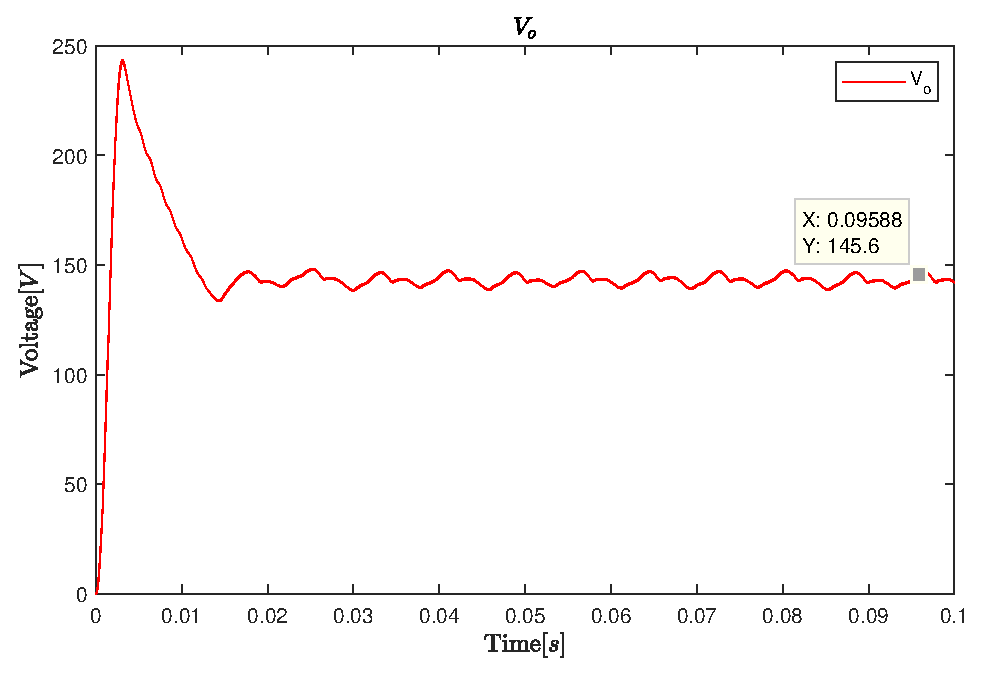
\includegraphics[width=\textwidth]{figures/yy2NxMultilevelBC/2Nx_SimResults.eps}
    \caption{2Nx Interleaved Boost Converter Voltage Output}
	\label{fig:MBC_2NxSimResult}
\end{figure}


\begin{figure}[H]
   \centering
   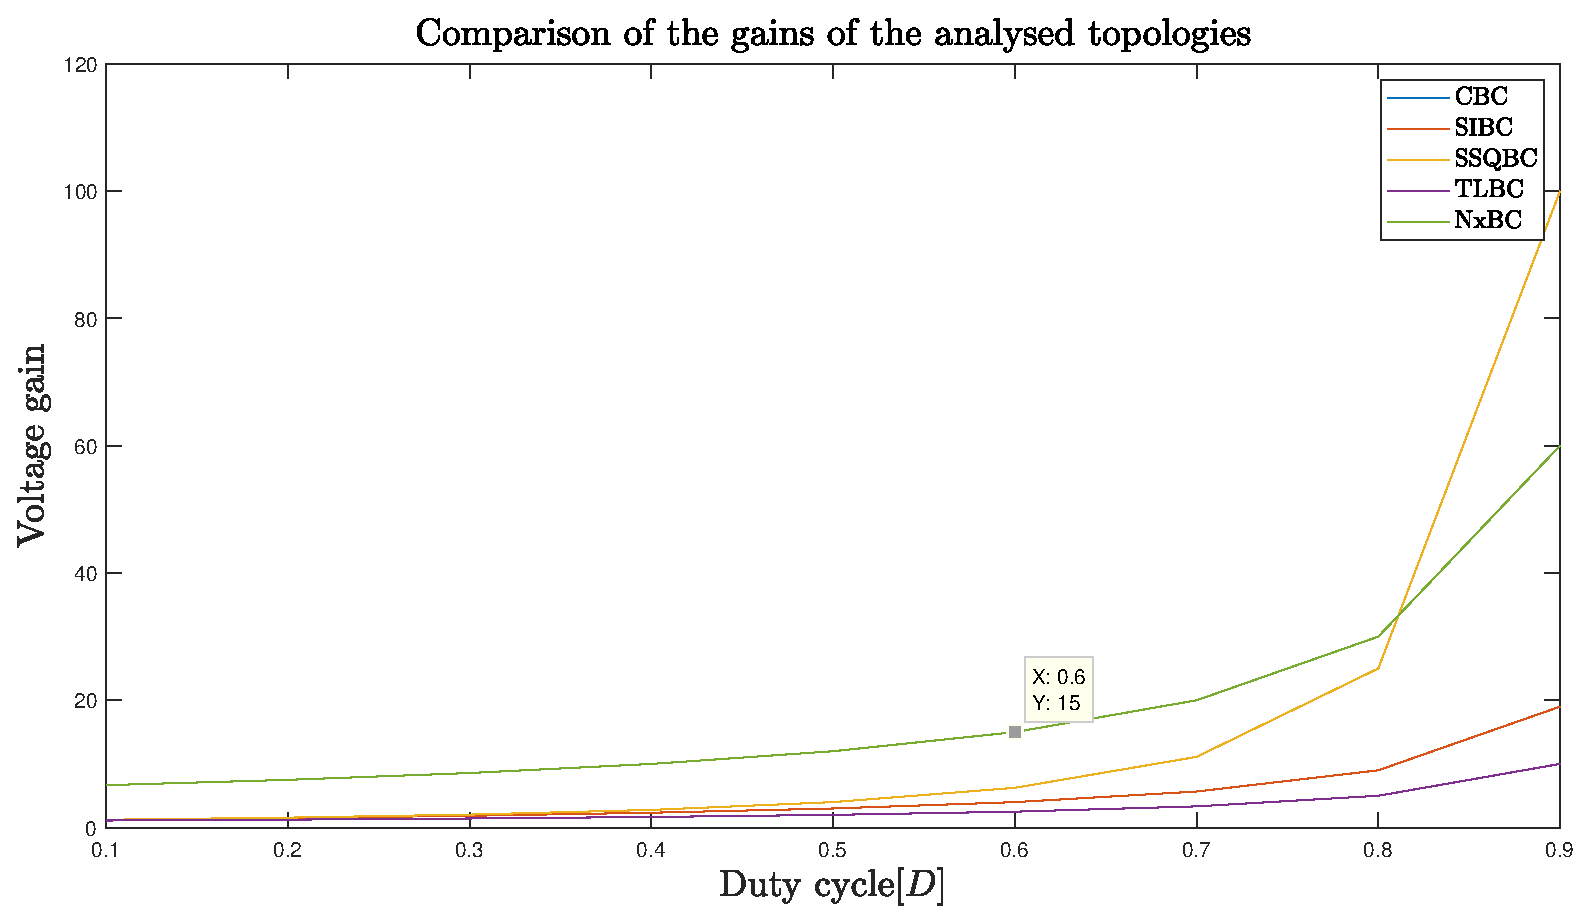
\includegraphics[width=\textwidth]{figures/gains.eps}
    \caption{2Nx Interleaved Boost Converter Voltage Output}
	\label{fig:MBC_2NxSimResult}
\end{figure}